\documentclass{article}

%other packages
\usepackage[a4paper]{geometry}
\usepackage{longtable}
\usepackage{wrapfig}
\setlength\parindent{0pt}
\usepackage{enumitem}
\usepackage[table]{xcolor}
\usepackage{polynom}
\def\scaleint#1{\vcenter{\hbox{\scaleto[3ex]{\displaystyle\int}{#1}}}}
\usepackage{array}
\newcolumntype{C}{>{{}}c<{{}}} % for '+' and '-' symbols
\newcolumntype{R}{>{\displaystyle}r} % automatic display-style math mode 
\usepackage{tabularray}
\usepackage{dcolumn,tabularx,booktabs}
\usepackage{esvect}

%maths
\usepackage{mathtools}
\usepackage{amsmath}
\usepackage{amssymb}
\usepackage{amsfonts}
\usepackage{autobreak}

%tikzpicture
\usepackage{tikz}
\usepackage{scalerel}
\usepackage{pict2e}
\usepackage{tkz-euclide}
\usepackage{tikz-3dplot}
\usetikzlibrary{calc}
\usetikzlibrary{patterns,arrows.meta}
\usetikzlibrary{shadows}
\usetikzlibrary{external}
\usetikzlibrary{decorations.pathreplacing,angles,quotes}
\usetikzlibrary{perspective,spath3}

%pgfplots
\usepackage{pgfplots}
\pgfplotsset{compat=1.18}
\usepgfplotslibrary{statistics}
\usepgfplotslibrary{fillbetween}

\pgfplotsset{
    standard/.style={
    axis line style = thick,
    trig format=rad,
    enlargelimits,
    axis x line=middle,
    axis y line=middle,
    enlarge x limits=0.15,
    enlarge y limits=0.15,
    every axis x label/.style={at={(current axis.right of origin)},anchor=north west},
    every axis y label/.style={at={(current axis.above origin)},anchor=south east}
    }
}

\begin{document}

Math 115 - Week 6, Class 14 - 16 Feb 2024
\hrule

\vspace{10pt}

As usual, Dr. Solomonovich began class by asking if anyone had any questions, and there was one.

\vspace{10pt}

{\bf{}QUESTION} How do you evaluate $\displaystyle\int\limits_3^4\frac{x^3-2x^2-4}{x^3-2x^2}\ dx$

\vspace{10pt}

The integrand is an improper irrational fraction, so we \textit{could} take the usual method of testing the denominator for a factor using the Factor Theorem, and then polynomially long-dividing the numerator by that factor and cancel terms to obtain a proper rational integrand. That being said, there's a trick here which makes it \textit{way} easier. We break up the fraction using the commutative property of addition, and optain an integrand which is a constant (1) plus a \textit{much} easier rational function.

\[\int\limits_3^4\frac{x^3-2x^2-4}{x^3-2x^2}\ dx=\int\limits_3^4\left(1-\frac{4}{x^2(x-2)}\right)\ dx\]

\vspace{10pt}

Now we use partial fractions to re-express the quotient as a sum of simpler fractions which are more easily integrable.

\begin{align*}
\frac{4}{x^2(x-2)}&=\frac{A}{x^2}+\frac{B}{x}+\frac{C}{x-2}\\
&=\frac{Ax-2A+Bx^2-2Bx+Cx^2}{x^2(x-2)}\\
&=\frac{(B+C)x^2+(A-2B)x-2A}{x^2(x-2)}
\end{align*}

\vspace{10pt}

Since we know the original coefficients, we can create a system of linear equations and solve for the undetermined coefficients.

\[\begin{aligned}x^2:\\x:\\1:\end{aligned}\left|\begin{aligned}B+C=0&\quad C=1\\A-2B=0&\quad B=A/2=-1\\-2A=4&\quad A=-2\end{aligned}\right.\]

\vspace{10pt}

And now we can re-espress the integrand in simpler terms;

\begin{align*}
\int\limits_3^4\left(1-\frac{4}{x^2(x-2)}\right)\ dx&=\int\limits_3^4\left(1-\left(\frac{-2}{x^2}+\frac{-1}{x}+\frac{1}{x-2}\right)\right)\ dx\\
&=x\Big|_3^4+\int\limits_3^4\frac{2}{x^2}\ dx+\int\limits_3^4\frac{1}{x}\ dx-\int\limits_3^4\frac{1}{x-2}\ dx\\
&=(4-3)+\frac{2x^{-1}}{-1}\Bigg|_3^4+\ln(x)\Big|_3^4-\ln(x-2)\Big|_3^4\\
&=1-\frac{1}{2x}\Bigg|_3^4+\ln4-\ln3-\ln2+\ln1\\
&=1-\frac{1}{8}+\frac{1}{6}+\ln\frac{2}{3}\\
&=\frac{23}{24}+\ln\frac{2}{3}
\end{align*}

\vspace{10pt}

And then we looked at the integral of the secant function. There are many ways to solve this, and frankly, Stewart's solution is so non-obvious that if he had proposed it 500 years ago, he probably would have been tried for witchcraft because only a supernatural entity like the devil could have revealed that information to him. We'll show his solution second.

\vspace{10pt}

{\bf{}SOLUTION 1:}

\begin{align*}
\int\frac{1}{\cos x}\ dx&=\left(\begin{aligned}\cos x\ dx=d\ \sin x\\\cos^2x+\sin^2x=1\end{aligned}\right)\\
&=\int\frac{\color{red}\boxed{\color{black}\cos x\ dx}}{\cos^2x}\\
&=\int\frac{1}{1-\sin^2x}\ d(\sin x)=(\sin x=u)\\
&=\int\frac{1}{1-u^2}\ du=-\int\frac{1}{u^2-1}\ du\\
&=-\frac{1}{2}\ln\left|\frac{u-1}{u+1}\right|+C\\
&=\frac{1}{2}\ln\left|\frac{u+1}{u-1}\right|+C\\
&=\frac{1}{2}\ln\left|\frac{\sin x+1}{\sin x-1}\right|+C\\
&*\mbox{Always non-negative}\\
&=\ln\sqrt{\frac{\sin x+1}{\sin x-1}}+C
\end{align*}

\newpage

{\bf{}SOLUTION 2:} (Stewart's)

\[\int\sec x\ dx=\int\sec x\cdot\frac{\sec x+\tan x}{\sec x+\tan x}\ dx\]

\vspace{10pt}

{\bf{}SOLUTION 3:} (Weierstrass (or, Universal) Substitution)

\vspace{10pt}

It is generally accepted among mathematicians that on top of being a brilliant mathematician, Karl Weierstrass, the founder of Analysis, was also a pretty decent human being. He was known for nurturing the development of young math talents without being envious of their capabilities - something I wish more mathematicians would take after. 

\vspace{10pt}

Dr. Solomonovich told me personally that there would be a question on the midterm which will require this integration technique. Though, since different people get different midterms, I'm not sure if everybody will get it or not. Most people get the same midterm, but some people get different ones for various reasons.

\vspace{10pt}

Weierstrass substitution converts integrals of rational functions of first-order trigonometric functions (ie. $\sin x$ and $\cos x$) into integrals of non-trigonometric rational functions which can be solved with partial fractions. It's a bit, how should I put it, (elaborate?), but it makes complete sense when you look at the problem generally. Essentially, we make a substitution which is based on a unit circle identity, and we just solve that identity for $x$, and derive the rational expressions for $\sin x$ and $\cos x$ based on trigonometric identities using the unit circle. I'll derive it for you (in the first quadrant) so the steps make sense, as they were not all shown in class.

\vspace{10pt}

We can start with using the "primitive" definition of the trig identites to get out bearings, then divide all sides by the length of the hypotenuse in order to get it to "fit" inside the unit circle. Do note that when using trigonometry in calculus, you must do it using the unit circle and not just with triangles, because triangles do not take into account non-acute central angles.

\[\mbox{Let }\tan\frac{x}{2}=t\]

\begin{center}
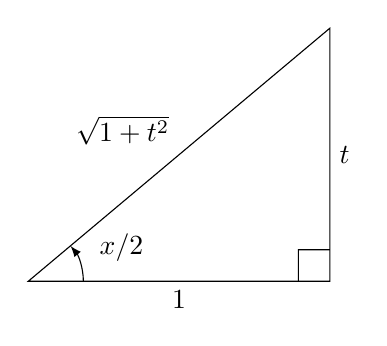
\begin{tikzpicture}[scale=5]
\coordinate (O) at (0,0);
\coordinate (P) at (40:1);
\coordinate (X) at (P |- O);
\draw[] (O) -- node[pos=0.5, above left]{$\sqrt{1+t^2}$} (P) -- node[pos=0.5, right]{$t$} (X) -- node[pos=0.5, below]{$1$} (O) -- cycle;
\draw pic["$x/2$",draw,-latex,angle eccentricity=1.8, angle radius=0.7cm]{angle=X--O--P};
\draw pic[draw,-,angle eccentricity=1.4, angle radius=0.4cm]{right angle=P--X--O};
\end{tikzpicture}
\end{center}

\begin{center}
\begin{tikzpicture}[scale=5]
\draw[] (0,0) circle [radius=1];
\coordinate (O) at (0,0);
\coordinate (P) at (40:1);
\coordinate (X) at (P |- O);
\draw[] (O) -- node[pos=0.5, above left]{$1$} (P) -- node[pos=0.5, right]{$\frac{t}{\sqrt{1+t^2}}$} (X) -- node[pos=0.5, below]{$\frac{1}{\sqrt{1+t^2}}$} (O) -- cycle;
\draw pic["$x/2$",draw,-latex,angle eccentricity=1.8, angle radius=0.7cm]{angle=X--O--P};
\draw pic[draw,-,angle eccentricity=1.4, angle radius=0.4cm]{right angle=P--X--O};
\end{tikzpicture}
\end{center}

\vspace{10pt}

Now that we know $\sin(x/2)$ and $\cos(x/2)$, we can use the double angle formulas (starting with cosine!) to easily express these without the linear factor inside the trigonometric functions.

\[\cos x=\frac{1}{1+t^2}-\frac{t^2}{1+t^2}=\frac{1-t^2}{1+t^2}\]

\[\sin x=2\cdot\frac{t}{\sqrt{1+t^2}}\cdot\frac{1}{\sqrt{1+t^2}}=\frac{2t}{1+t^2}\]

\vspace{10pt}

This lets us use the following substitution;

\begin{align*}
\int\frac{1}{\cos x}\ dx&=\left(\begin{aligned}\tan\frac{x}{2}=t\quad\frac{x}{2}=\arctan t\\\ dx=\frac{2\ dt}{1+t^2}\\\sin x=\frac{2t}{1+t^2}\quad\cos x=\frac{1-t^2}{1+t^2}\end{aligned}\right)\\
&=\int\frac{1+t^2}{1-t^2}\cdot\frac{2\ dt}{1+t^2}\\
&=2\int\frac{dt}{1-t^2}\\
&=2\cdot\frac{-1}{2}\ln\left|\frac{t-1}{t+1}\right|+C\\
&=\ln\left|\frac{t+1}{t-1}\right|+C\\
&=\ln\left|\frac{\tan\frac{x}{2}+1}{\tan\frac{x}{2}-1}\right|+C
\end{align*}

\vspace{10pt}

{\bf{}HOMEWORK} Use Weierstrass Substitution to solve $\displaystyle\int\csc x\ dx$

\vspace{10pt}

{\bf{}HOMEWORK} Evaluate $\displaystyle\int\frac{1}{2+\cos x}\ dx$ using Weierstrass Substitution

\vspace{10pt}

{\bf{}EXAMPLE} Evaluate $\displaystyle\int\sin^3x\ dx$

\begin{align*}
\int\sin^3x\ dx&=\int\sin^2x\cdot\sin x\ dx\\
&=\left(\begin{aligned}\cos x=t\\-\sin x\ dx=\ dt\\\sin x\ dx=\ -dt\\\sin^2x=1-t^2\end{aligned}\right)\\
&=-\int(1-t^2)\ dt=-t+\frac{t^3}{3}+C\\
&=-\cos x+\frac{1}{3}\cos^2x+C
\end{align*}

\newpage

{\bf{}EXAMPLE} Evaluate $\displaystyle\int\frac{\sin x+\cos x}{\sin x-\cos x}\ dx$ (we do it without Weierstrass, but that works too)

\begin{align*}
\int\frac{\sin x+\cos x}{\sin x-\cos x}\ dx&=\int\frac{\tan x+1}{\tan x-1}\ dx\\
&=\left(\begin{aligned}\tan x=u\\x=\arctan u\\dx=\frac{1}{1+u^2}\ du\end{aligned}\right)\\
&=\int\frac{u+1}{u-1}\cdot\frac{1}{1+u^2}\ du\\
&=\mbox{partial fractions, etcettera}\\
\end{align*}

\vspace{10pt}

We will decompose the integrand into the sum of its partial fractions.

\begin{align*}
\frac{u+1}{(u-1)(u^2+1)}&=\frac{A}{u-1}+\frac{Bu+C}{u^2+1}\\
&=\frac{Au^2+A+Bu^2-Bu+Cu-C}{(u-1)(u^2+1)}\\
&=\frac{(A+B)u^2+(-B+C)u+(A-C)}{(u-1)(u^2+1)}
\end{align*}

\[\left.\begin{aligned}u^2:\\u:\\1:\end{aligned}\right|\left.\begin{aligned}A+B=0\\-B+C=1\\A-C=1\end{aligned}\right\}\begin{aligned}2A=2\quad\boxed{A=1}\\\boxed{B=-1}\\\boxed{C=A-1=0}\end{aligned}\]

\vspace{10pt}

So, we are left with an easily integrable function. In a humorous way, I would mention that we can spend ages simplifying the resulting indefinite integral using trigonometric identities.

\begin{align*}
\int\frac{u+1}{(u-1)(u^2+1)}\ du&=\int\frac{1}{u-1}-\frac{u}{u^2+1}\ du\\
&=\ln|u-1|-\frac{1}{2}\ln(u^2+1)+C\\
&=\ln\left|\frac{u-1}{\sqrt{u^2+1}}\right|+C\\
&=\ln\frac{|\tan x-1|}{\sqrt{\sec^2x}}+C\\
&=\ln|\cos x(\tan x-1)|+C\\
&=\ln|\sin x-\cos x|+C
\end{align*}


\end{document}



